% !TEX root = SystemTemplate.tex

\chapter{Overview and concept of operations}

The overview should take the form of an executive summary.  Give the reader a feel 
for the purpose of the document, what is contained in the document, and an idea 
of the purpose for the system or product. 


\section{Scope}
What scope does this document cover? 


\section{Purpose}
What is the purpose of the system or product? 


\subsection{Major System Component \#1}
Describe briefly the role this major component plays in this system. 

\subsection{Major System Component \#2}
Describe briefly the role this major component plays in this system. 

\subsection{Major System Component \#3}
Describe briefly the role this major component plays in this system. 

\section{Systems Goals}
Briefly describe the overall goals this system plans to achieve.  These goals are 
typically provided by the stakeholders.  This is not intended to be a detailed 
requirements listing.  Keep in mind that this section is still part of the Overview. 

\section{System Overview and Diagram}
Provide a more detailed description of the major system components without getting 
too detailed.  This section should contain a high-level block and/or flow diagram 
of the system highlighting the major components.   See Figure~\ref{systemdiagram}.    This is a floating figure environment.  \LaTeX\ will try to put it close to where it was typeset but will not allow the figure to be split if moving it can not happen.   Figures, tables, algorithms and many other floating environments are automatically numbered and placed in the appropriate type of table of contents.  You can move these and the numbers will update correctly.

\begin{figure}[tbh]
\begin{center}
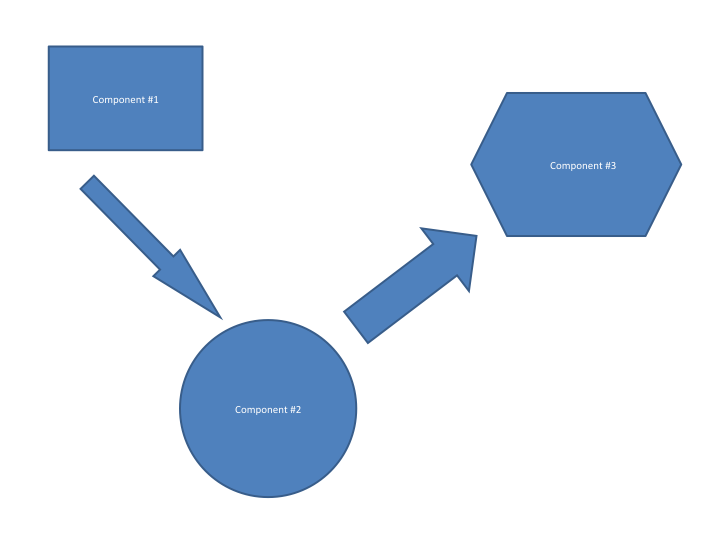
\includegraphics[width=0.75\textwidth]{./diagram}
\end{center}
\caption{A sample figure .... System Diagram \label{systemdiagram}}
\end{figure}

\section{Technologies Overview}
This section should contain a list of specific technologies used to develop the 
system.  The list should contain the name of the technology, brief description, 
link to reference material for further understanding, and briefly how/where/why 
it was used in the system.    See Table~\ref{somenumbers}.  This is a floating table environment.  \LaTeX\ will try to put it close to where it was typeset but will not allow the table to be split.   
\begin{table}[tbh]
\begin{center}
\begin{tabular}{|r|l|}
  \hline
  7C0 & hexadecimal \\
  3700 & octal \\ \cline{2-2}
  11111000000 & binary \\
  \hline \hline
  1984 & decimal \\
  \hline
\end{tabular}
\caption{A sample Table ... some numbers. \label{somenumbers}}
\end{center}
\end{table}

